\addcontentsline{toc}{chapter}

\chapter{Introduction}

Mitochondria is a membrane bound cell organelle in eukaryotes which appear to be fundamental to all eukaryotes.  They are involved in various metabolic processes of a cell, like the citric acid cycle, creating lipids such as cardiolipin, making essential protein cofactors of proteins like Fe-S clusters, they are the site of cellular respiration and the electron transport chain that generate ATP. The name 'Mitochondrion' is termed from 'mito' and 'chondrion' which translate to 'beads' and 'strings' an analogy made to describe their shape within cells. Mitochondria are very dynamic organelles, constantly fragmenting and fusing in a network through the cell, even transporting to far ends of neurons, along the cytoskeleton. 
\\
\begin{wrapfigure}{r}{}
  \begin{center}
    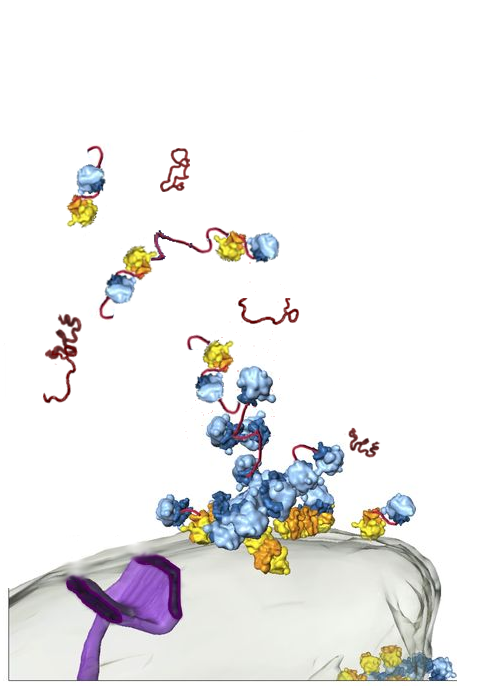
\includegraphics[width=0.4\textwidth]{Mitotransimport}
  \end{center}
  \caption{Selectively translated mRNA by heterogenous ribosomes}
  \label{selectivelytranslatedmrna}
\end{wrapfigure}

For it’s diverse role within the eukaryotic cell, its history is rooted in the kingdom prokaryota. It is considered to once have been an independent organism. Proof of the endosymbiotic theory of mitochondrial origin finally came into existence with the evidence of Mitochondria hosting it’s own DNA\textsuperscript{\cite{Gerst}}.
\vspace{3cm}



\clearpage

\paragraph{Some tips on how to use \LaTeX are here below:}
\newline
A cool experiment i tried is here (Sec:\ref{hefetrafo}), you should check it out.
\\
\vspace{2cm}

sometimes it helps to make \hspace{5mm} spaces...

\newline

The last page has a cool image I made using MS Paint: (Fig:\ref{selectivelytranslatedmrna}).

\paragraph{Accents and shit:}

Can you pronounce these?: \newline
{\"a} {\^e} {\`i} {\.I} {\o} {\'u} {\aa} {\c c} {\u g} {\l} {\~n} {\H o} {\v r} {\ss}
\\
\newline
Check out this \textit{\underline{\href{https://www.overleaf.com/learn/latex/List_of_Greek_letters_and_math_symbols#Greek_letters}{link}}} for how to write greek letters.
And this  \textit{\underline{\href{https://www.overleaf.com/learn/latex/Bold,_italics_and_underlining#Italicized_text}{link}}} about basic text formatting.\\
